\documentclass[dvipdfmx,fleqn]{beamer}
\usepackage{amsmath,amsthm,amssymb}
\usepackage{algorithm,algpseudocode}
\graphicspath{{./figure/}{./plot/}}
\makeatletter
\def\input@path{{./figure/}{./table/}}
\makeatother
\usepackage[
style=ieee,backend=bibtex,
texencoding=utf8,bibencoding=utf8,
dashed=false,
isbn=false,url=false,doi=false,
sorting=debug
]{biblatex}
\addbibresource{References.bib}
\AtBeginBibliography{}
\setbeamertemplate{bibliography item}[text]
\usetheme{IMELAB}
\usefonttheme[onlymath]{serif}

\usepackage{bxdpx-beamer}
\usepackage{pxjahyper}
\usepackage{verbatim}
%\usepackage[absolute,overlay]{textpos}

\renewcommand{\kanjifamilydefault}{\gtdefault}
\renewcommand{\familydefault}{\sfdefault}

% Theorem
\uselanguage{japanese}
\languagepath{japanese}
\deftranslation[to=japanese]{Theorem}{定理}
\deftranslation[to=japanese]{Lemma}{補題}
\deftranslation[to=japanese]{Example}{例}
\deftranslation[to=japanese]{Examples}{例}
\deftranslation[to=japanese]{Definition}{定義}
\deftranslation[to=japanese]{Definitions}{定義}
\deftranslation[to=japanese]{Problem}{問題}
\deftranslation[to=japanese]{Solution}{解}
\deftranslation[to=japanese]{Fact}{事実}
\deftranslation[to=japanese]{Proof}{証明}
\def\proofname{証明}

% Caption
\renewcommand{\figurename}{図}
\renewcommand{\tablename}{表}

% Beamer Misc.
\usepackage{appendixnumberbeamer}
\setbeamertemplate{navigation symbols}{}
\setbeamertemplate{frametitle continuation}[from second][(続き)]
\setbeamertemplate{section in toc}{\hspace{0.75em}\usebeamercolor[fg]{itemize item}$\blacktriangleright$\hspace{.5em}\usebeamercolor[fg]{normal text}\inserttocsection \\}
\setbeamertemplate{subsection in toc}{\hspace{2em}\usebeamercolor[fg]{itemize item}\inserttocsubsectionnumber\hspace{.5em}\usebeamercolor[fg]{normal text}\inserttocsubsection \\}
\newenvironment{enumalgo}{\begin{enumerate}\scriptsize\setlength\itemsep{0ex}\setlength\leftmargini{0ex}\setlength\leftmarginii{1em}\setlength\leftmarginiii{1em}}{\end{enumerate}}

\title[媒介中心性更新法]{辺操作時の最短経路の更新を利用する \\ 媒介中心性の更新法}
\author[里谷]{里谷 佳紀}
\institute[情数工研]{情報数理工学研究室}
\date[試問]{\alert{試問の名前をかいてね} \\ 2020年2月12日}

\begin{document}

\makeIMELABtitle

\section{背景・目的}
\begin{frame}[t]{研究背景}
  \begin{itemize}
  \item \alert{媒介中心性}\footcite{01Freeman1977}:ネットワークの頂点の重要度を示す.
  \item[] 鉄道網における駅,社会ネットワークにおける人など
  \end{itemize}
  \begin{columns}[T]
    \begin{column}{.49\textwidth}
      \begin{itemize}
      \item[] \begin{equation*}
        B_v=\sum_{s\neq v}\sum_{t\neq v,s}\frac{\sigma_{st}(v)}{\sigma_{st}}.
      \end{equation*}
        \begin{itemize}
        \item $\sigma_{st}$:$s$と$t$間の最短経路の数,
        \item $\sigma_{st}(v)$:$s$と$t$間の最短経路の内$v$を通るものの数.
        \end{itemize}
        \medskip
      \item 媒介中心性が高い\\$\rightarrow$多くの最短経路が通る
      \end{itemize}
    \end{column}
    \begin{column}{.49\textwidth}
      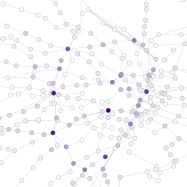
\includegraphics[width=.9\columnwidth]{tokyo.pdf}
    \end{column}
  \end{columns}
\end{frame}

\begin{frame}{媒介中心性の計算例}
  \vspace{-2em}
  \begin{columns}
    \begin{column}{.6\textwidth}
      \begin{flalign*}
        B_v&=\sum_{s\neq v}\sum_{t\neq s,v}\frac{\sigma_{st}(v)}{\sigma_{st}}\\
        &=\frac{\sigma_{wx}(v)}{\sigma_{wx}}+\frac{\sigma_{wy}(v)}{\sigma_{wy}}
        +\frac{\sigma_{wz}(v)}{\sigma_{wz}}\\
        &+\frac{\sigma_{xy}(v)}{\sigma_{xy}}+\frac{\sigma_{xz}(v)}{\sigma_{xz}}
        +\frac{\sigma_{yz}(v)}{\sigma_{yz}}+\cdots\\
        &=\frac{0}{1}+\frac{0}{1}+\frac{1}{1}+\frac{0}{1}+\frac{2}{2}+\frac{1}{1}\cdots\\
        &=6
      \end{flalign*}
      同様に,$B_w=B_y=2,\:B_x=B_z=0$.
    \end{column}
    \begin{column}{.39\textwidth}
      \centering
      \def\svgwidth{.9\linewidth}
      \input{graph-bc.pdf_tex}
    \end{column}
  \end{columns}
\end{frame}

\begin{frame}{Brandesのアルゴリズム}
  \alert{TODO}
\end{frame}

\begin{frame}{関連研究}
  \alert{TODO}
\end{frame}

\begin{frame}{研究目的}
  \alert{TODO}
\end{frame}

\section{提案アルゴリズム}
\begin{frame}{アルゴリズムの概要}
  \begin{itemize}
  \item 基本アイデア:既存の二つの方法を応用
    \begin{itemize}
    \item RamalingamとRepsの最短経路更新法
    \item Bergaminiらの媒介中心性更新法
    \end{itemize}
  \end{itemize}
  \begin{itemize}
  \item 記号
    \begin{itemize}
    \item $s$から$t$への最短経路長:$d_{st}$(削除後は$d'_{st}$)
    \item $s$から$t$への最短経路数:$\sigma_{st}$(削除後は$\sigma'_{st}$)
    \item $s$と$v$のペア依存度:$\delta_{s}(v)$(削除後は$\delta'_{s}(v)$)
    \item $v$の媒介中心性:$B_v$(削除後は$B'_v$)
    \end{itemize}
  \end{itemize}
\end{frame}

\begin{frame}{影響を受ける頂点}
  \alert{TODO}
\end{frame}

\begin{frame}{媒介中心性更新 -- 変化量の定義}
  \alert{TODO}
\end{frame}

\begin{frame}{媒介中心性更新 -- 変化量の計算}
  \alert{TODO}
\end{frame}

\begin{frame}{最短経路更新 -- \alert{挿入時}}
  \alert{何かしら}
\end{frame}

\begin{frame}{最短経路更新 -- \alert{削除時}}
  \alert{何かしら}
\end{frame}

\begin{frame}{時間計算量の解析}
  \alert{TODO}
\end{frame}

\section{数値実験}
\begin{frame}{数値実験}
  \alert{TODO}
\end{frame}

\begin{frame}{性能比較}
  \alert{TODO}
\end{frame}

\begin{frame}{計算量の検証}
  \alert{TODO}
\end{frame}

\begin{frame}{道路ネットワークへの応用}
  \alert{TODO}
\end{frame}

\section{まとめ}
\begin{frame}{まとめ}
  \alert{TODO}
\end{frame}

\appendix
\section{参考文献}
\begin{frame}[allowframebreaks]{参考文献}
  \printbibliography[title=]
\end{frame}

\end{document}
